%\part{Konstruktion}

\chapter{Programmlogik}
Unter dem Punkt Programmlogik wird der ganze Anfrageprozess verstanden. Dieser reicht vom Extrahieren von \lstinline|SearchModel|s bis hin zum Ausliefern der \lstinline|SearchResult|s stützt sich auf folgende wichtige Komponenten:

\begin{enumerate}
     \item \lstinline|SEARCHExtraction|
     \item \lstinline|QueryCreation|
     \item \lstinline|QueryResolution|
     \item \lstinline|Ranking|
\end{enumerate}

\begin{figure}[htb]
  \centering
  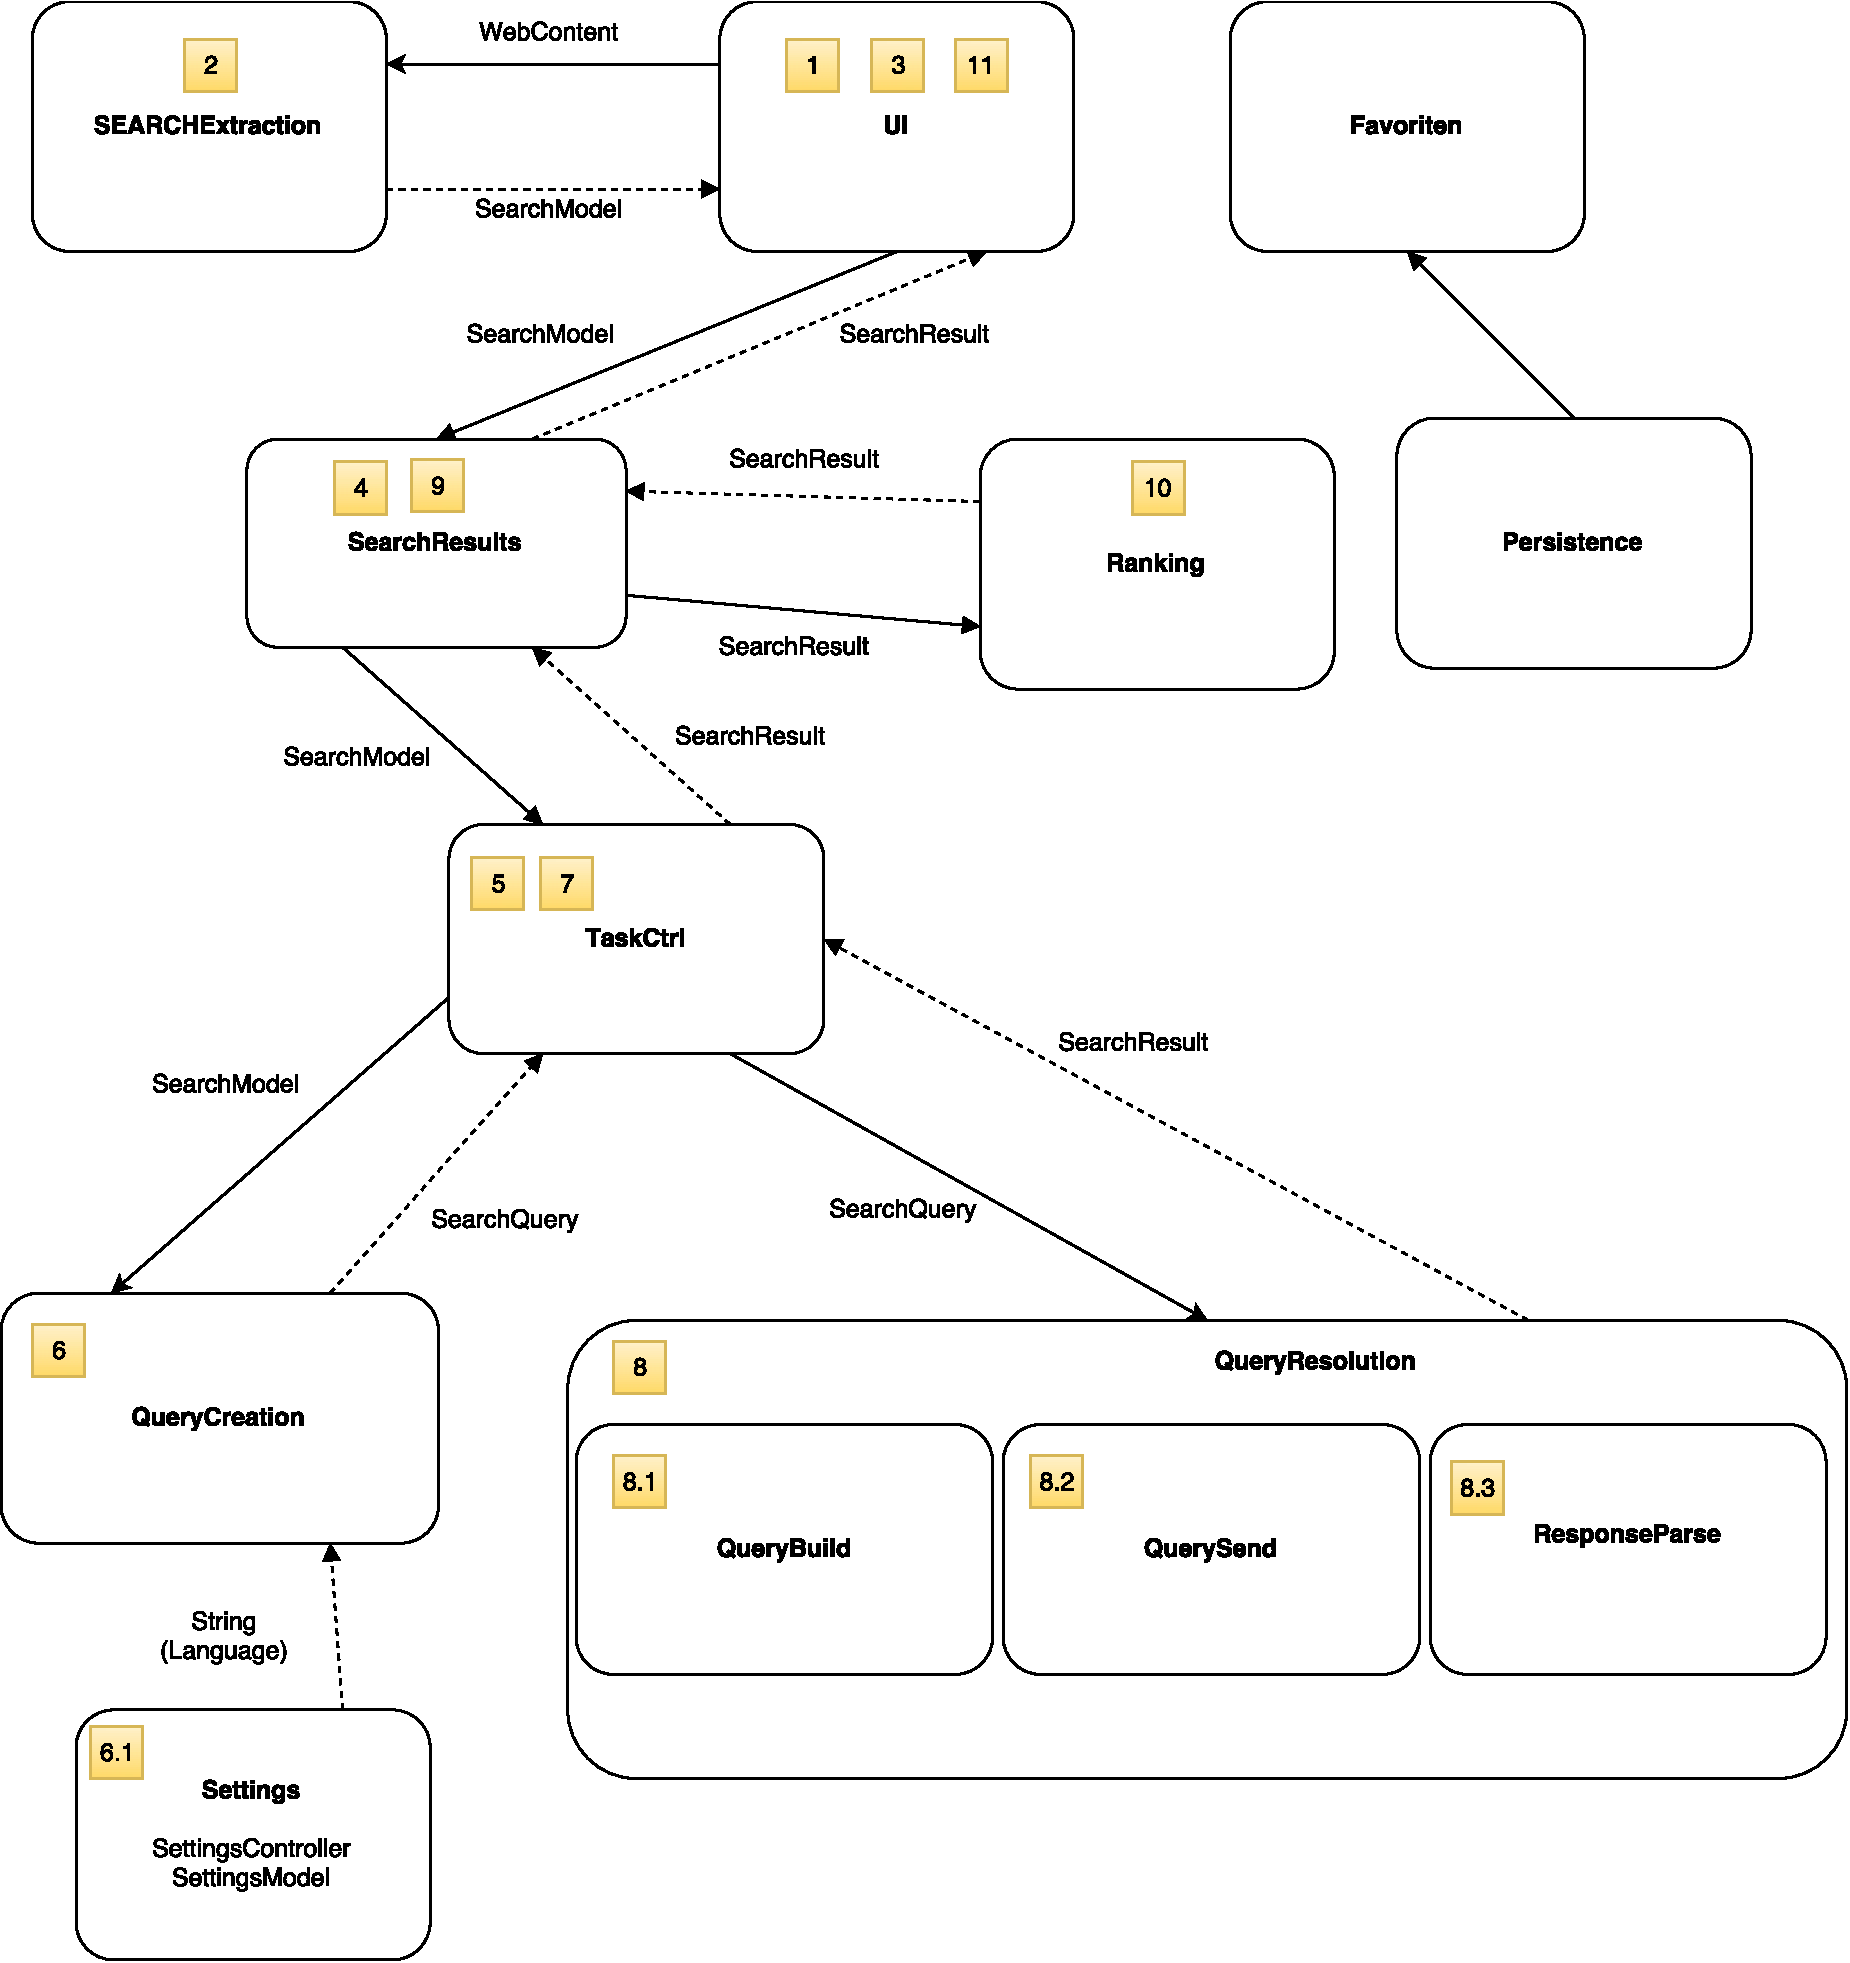
\includegraphics[width=\textwidth]{Architektur}
  \caption{Übersicht des Kapitels Programmlogik}
\end{figure}

Im Folgenden werden alle Teile der Programmlogik beschrieben.

%\part{Konstruktion}
%\chapter{Programmlogik}

\section{TaskCtrl}

Der \lstinline|TaskCtrl| ist einer der wichtigsten Elemente bei der Kommunikation zwischen der Oberfläche und dem Abrufen der Daten aus dem Internet. Er bestimmt mit Hilfe der vom Nutzer getroffenen Einstellungen an welche Suchmaschine die Anfrage geschickt wird. Die Einstellungen werden durch das \lstinline|Settings.bundle| definiert und können durch die Klasse \lstinline|SettingsManager| abgerufen werden. 

Der \lstinline|TaskCtrl| wird von der Klasse \lstinline|SearchResults| initialisiert und aufgerufen. Zuerst werden unter Verwendung der Klasse \lstinline|QueryCreationCtrl| Daten in einem allgemeingültigen Format für die Suchanfragen erstellt. Diese Daten werden daran anschließend von den jeweiligen \lstinline|QueryBuildern| (\lstinline|EEXCESSJSONBuilder|, \lstinline|DuckDuckGoURLBuilder| und \lstinline|FarooURLBuilder|) in das für die jeweilige Suchmaschine passende Datenformat umgewandelt. Die Suchanfragen werden asynchron durch die entsprechenden \verb|ConnectionCtrl| (\lstinline|JSONConnectionCtrl| und \lstinline|URLConnectionCtrl|) versendet. Bei erfolgreicher Suche und nach erfolgreichem Parsen der Ergebnisse werden diese dann mit Aufruf der Methode \lstinline|setRecommendation(|\lstinline|status:String,| \lstinline|message:String,| \lstinline|result:SearchResult)| an den Aufrufer, die Klasse \lstinline|SearchResults|, zurückgegeben. Diese speichert die Suchergebnisse in einem Cache zwischen. Der \lstinline|TaskCtrl| wird nur aufgerufen, falls zu dem jeweiligen \SEARCH-Tag noch keine Ergebnisse im Cache vorhanden sind. 

%\subsection{Teilabschnitt}
%\subsubsection{Unterteilabschnitt}
%\paragraph{Paragraph}
%\subparagraph{Unterparagraph}

%\begin{sloppy}

%\part{Konstruktion}
%\chapter{Programmlogik}

\section{SEARCHExtraction}

\subsection{SearchManager}
\subsection{RegexForSEARCH}

%\subsubsection{Unterteilabschnitt}
%\paragraph{Paragraph}
%\subparagraph{Unterparagraph}

%\part{Konstruktion}
%\chapter{Programmlogik}

\section{SEARCHModels}
Das SearchModels stellt die Schnittstelle zwischen der SearchExtraction und dem TaskController dar. Von der SearchExtraction erzeugt beinhaltet ein SearchModels-Objekt eine Sammlung von SearchModel-Objekten erzeugt aus einer Website. In einem SearchModel-Objekt werden Search-Tag-Links mit der zugehörigen Search-Tag-Section/-Head und Filtern gespeichert.\newline
Zur globalen Identifikation wird in einem SearchModel die Url der Website von der es kommt gesetzt. Um ein SearchModel innerhalb einer Seite zu finden wir der Index gesetzt.

%\subsection{Teilabschnitt}
%\subsubsection{Unterteilabschnitt}
%\paragraph{Paragraph}
%\subparagraph{Unterparagraph}

%\part{Konstruktion}
%\chapter{Programmlogik}

\section{QueryCreation}

\begin{figure}[htb]
   \centering
  	\includegraphics[width=0.4\textwidth]{QueryCreation}
  	\caption{Aufbau des Moduls \lstinline|QueryCreation|}
\end{figure}
\lstinline|QueryCreation| generiert aus den Suchwörtern (\lstinline|SearchModel|) und den Geräte- und App-Einstellungen ein allgemeines Anfrageformat. Dieses Anfrageformat wird in \lstinline|QueryResolution| zu einem für jede Suchmaschine spezifischen Suchformat umgewandelt.

\subsection{QueryCreationCtrl}

%\subsubsection{Unterteilabschnitt}
%\paragraph{Paragraph}
%\subparagraph{Unterparagraph}

%%\part{Konstruktion}
%\chapter{Programmlogik}

\section{SearchQuerys}
%\part{Konstruktion}
%\chapter{Programmlogik}

\section{QueryResolution}

\begin{figure}[htb]
  	\includegraphics[width=\textwidth]{qr_querysend.png}
  	\caption{Aufbau des Moduls QueryResolution}
	\label{fig:Aufbau des Moduls QueryResolution}
\end{figure}

%\part{Konstruktion}
%\chapter{Programmlogik}
%\section{QueryResolution}

\subsection{JSONData}

%\paragraph{Paragraph}
%\subparagraph{Unterparagraph}

\newpage
%\part{Konstruktion}
%\chapter{Programmlogik}
%\section{QueryResolution}

\subsection{QueryBuild}

Das Modul QueryBuild liefert den größten Teil der Intelligenz im Modul QueryResolution. Die Aufgaben des Moduls sind es, die ConnectionController in QuerySend zu konfigurieren, die Query in das suchmaschinenspezifische Anfrageformat umzuwandeln und dem ConnectionController den Parser für die Antwort zu geben.

Es gibt für jede Suchmaschine eine Implementation der Spezifikation AbstractBuilder, welche durch die Spezifikationen URLAbstractBuilder und JSONAbstractBuilder erweitert wird.

\subsubsection{AbstractBuilder}
\subsubsection{AbstractJSONBuilder}
\subsubsection{AbstractURLBuilder}
\subsubsection{EexcessJSONBuilder}
\subsubsection{FarooURLBuilder}
\subsubsection{DuckDuckGoURLBuilder}
\subsubsection{EEXCESSOrigin}

%\paragraph{Paragraph}
%\subparagraph{Unterparagraph}

\newpage
%\part{Konstruktion}
%\chapter{Programmlogik}
%\section{QueryResolution}

\subsection{QuerySend}

\begin{figure}[htb]
	\centering
  	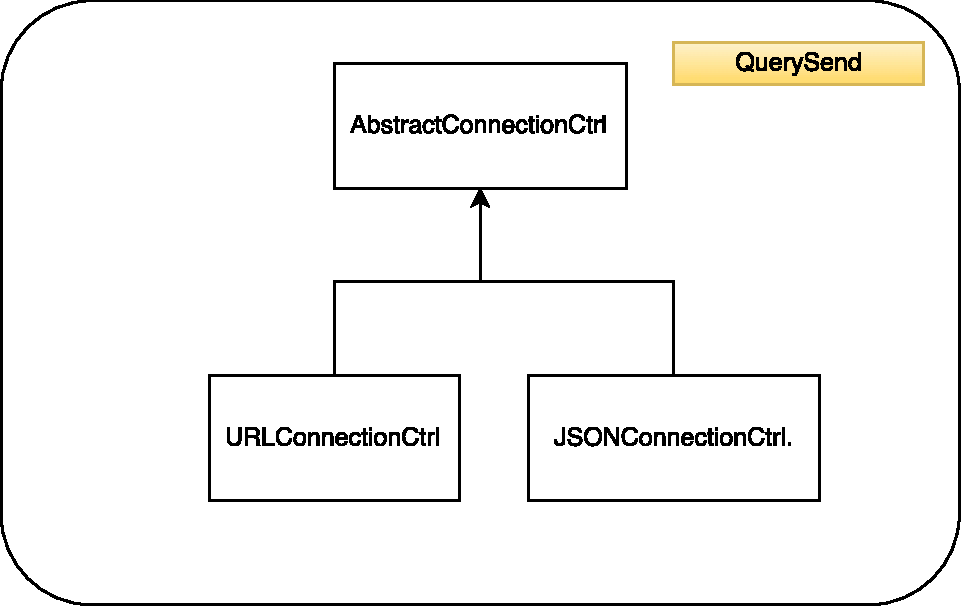
\includegraphics[width=0.8\textwidth]{qr_querysend}
  	\caption{Aufbau des Moduls \lstinline|QuerySend|}
\end{figure}

Im Modul \lstinline|QuerySend| befinden sich die \lstinline|ConnectionController|, die für das Versenden der Anfrage zuständig sind. Sie werden mithilfe von \lstinline|QueryBuild| konfiguriert und erhalten den Parser (\lstinline|ResponseParse|). Vor dem Weiterreichen an den \lstinline|TaskController|, wird durch den Parser noch von NSData zu \lstinline|SearchResult| umgewandelt.
\newpage
%\part{Konstruktion}
%\chapter{Programmlogik}
%\section{QueryResolution}

\subsection{ResponseParse}
\begin{figure}[htb]
	\centering
		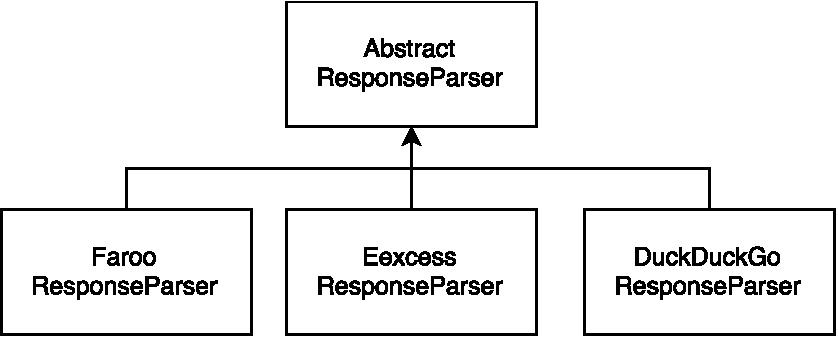
\includegraphics[]{response_parser}
		\caption{Aufbau des Moduls ResponseParse}
		\label{fig:Aufbau des Moduls ResponseParse}
\end{figure}
Der \lstinline|ResponeParser| ist für das Parsen der Antworten der Suchmaschinen in ein allgemeines Format.
Dabei wird in der aktuellen Version zwischen drei Parsern unterschieden.
\subparagraph{FarooResponseParser}
Hier werden die Antworten von Faroo verarbeitet.
\subparagraph{DuckDuckGoResponseParser}
Hier werden die Antworten von DuckDuckGO verarbeitet.
\subparagraph{EexcessResponseParser}
Hier werden die Antworten von Eexcess verarbeitet.
\subparagraph{AbstractResponseParser}
Der \lstinline|AbstractResponseParser| spezifiziert wie die untergeordneten \lstinline|ResponeParser| implementiert werden.

%\paragraph{Paragraph}
%\subparagraph{Unterparagraph}




%\paragraph{Paragraph}
%\subparagraph{Unterparagraph}

%\part{Konstruktion}
%\chapter{Programmlogik}

\section{SearchResults}
\begin{figure}[htb]
  \centering
  \includegraphics[width=0.4\textwidth]{SearchResults2}
  \caption{Ablaufmöglichkeiten im \lstinline|SearchResults|}
\end{figure}

\lstinline|SEARCHResults| ist ein Container, der für ein Suchwort die Suchergebnisse speichert.
Der Container ist in der Lage, bei fehlenden Suchergebnissen Suchanfragen abzuschicken und informiert mit dem Observer, ob neue Suchergebnisse von der Suchmaschine gekommen sind. Der Observer wird im \lstinline|PopViewController| registriert und ist somit in der Lage auf neue Suchergebnisse zu reagieren. 
%\subsection{Teilabschnitt}
%\subsubsection{Unterteilabschnitt}
%\paragraph{Paragraph}
%\subparagraph{Unterparagraph}

\pagebreak
%\part{Konstruktion}
%\chapter{Programmlogik}

\section{Ranking}
\subsection{Rules}
\subsection{SearchRules}
\subsection{RankingPersistence}
\subsubsection{PersistenceController}
\subsubsection{RankingDataObject}
\subsubsection{RankingDataObjectPersistency}

%\paragraph{Paragraph}
%\subparagraph{Unterparagraph}

\section{SettingsModel}
Im SettingsModel werden die verschiedenen Einstellungen für den Browser gespeichert.
Der Nutzer kann diese über das Einstellungsmenü des Geräts ändern.

\paragraph{Einstellungen}  

Die Einstellungen sind in drei verschiedene Kategorien eingeteilt.
\begin{itemize}  
     \item Suchmaschinen  
     \item Nutzerprofil
     \item Browsereinstellungen
\end{itemize}

\subparagraph{Suchmaschinen}  

Hier kann der Nutzer die verschiedenen Suchmaschinen einstellen, die für die SearchTags verwendet werden sollen.
Dabei kann entweder jede Suchmaschine einzeln gewählt werden, oder den Empfehlungen des Autors gefolgt werden.
Zur Auswahl stehen:
\begin{itemize}  
     \item DuckDuckGo
     \item Eexcess
     \item Faroo  
\end{itemize}
Sobald eine Suchmaschine gewählt wurde, werden die Empfehlungen des Autors ignoriert.

\subparagraph{Nutzerprofil}  
Hier können die Nutzerdaten angegeben werden.
Davon wird bisher nur die Sprach verwendet.
Einstellungsmöglichkeiten:
\begin{itemize}  
     \item Name  
     \item Alter  
     \item Stadt
     \item Land
     \item Sprache
\end{itemize}

\subparagraph{Startseite}  
Hier kann die Startseite des Browser festgelegt werden.
Die hier gesetzte Seite wird nocht nicht im Browser als Startseite übernommen.

